\chapter{Roadpricing}
\label{ch:roadpricing}
% ##################################################################################################################

\hfill \textbf{Author:} Kai Nagel

\begin{center} 
\includegraphics[width=0.25\textwidth, angle=0]{figures/MATSimBook.png} \end{center}

\createStandardInformation{roadpricing}{\lstinline{RunRoadPricingExample} class}{roadpricing}%
{\citet{RieserBeuckNagel2007early-toll-zrh-etc,RieserEtAl_TRBTDF_2008,GretherEtAl_ERSA_2008}}

% ##################################################################################################################
\section{Introduction}
\label{sec:roadpricing-intro}
Roadpricing is an often-discussed policy measure \citep[e.g.,][]{ButtonVerhoef_1998}. Its implementation in \gls{matsim} is conceptually straightforward \citep{%
%
%RieserEtAl_TechRep_VSP_2007,%
RieserBeuckNagel2007early-toll-zrh-etc,%
RieserEtAl_TRBTDF_2008,%
GretherEtAl_ERSA_2008%
%
}: Essentially, for each vehicle entering a link at a given time, the appropriate toll is computed, and charged to the vehicle's driver. The scoring function will pick this up by the term (cf.\ Equation~(\ref{eq:tdisutility}))
\[
S_{trav,car,q} = ... + \beta_{c} \cdot (- \tau) + ... \ ,
\]
where $\tau$ is the sum of all toll payments, and $\beta_{c}$ is the marginal utility of money (also see Chapter~\ref{ch:economicEval}). The driver then takes this into account for decision-making, e.g.,\,with respect to route choice, departure time choice, mode choice, destination choice, etc., trading off toll payments with other elements of his or her scoring function.

It should be clear that this picks automatically up all kinds of heterogeneities, for example:
\begin{compactitem}
\item Traveling at a different time may lead to a different toll, but possibly also to different schedule delay costs (Section~\ref{sec:schedule-delay-costs}). 
% \kai{wo wird das mit dem schedule delay erklärt?}
\item Different vehicle types may be charged different tolls \citep{KickhoeferNagel2012EmissionInternalization}.
\item Different travelers may have different values of time \citep{NagelKickhoeferJoubert2014HeterogeneousVoTsPROCEDIA}, which may even vary by time-of-day.
\end{compactitem}

A challenge is, however, that the innovative modules (cf.~Section~\ref{sec:strategymodules}) need to be consistent with the scoring that is now modified by the road pricing: The approach described so far will not work if, say, the router consistently generates toll avoiding routes for a synthetic person with a high value of time who normally would want to pay money for a faster option---since, if a suitable route is never generated, then the scoring has no chance to identify it and thus the choice process has no chance to select it in subsequent iterations.

However, passing all details of an individual, i.e.,\,not only the marginal utility of money but also the specific time pressure at the time of the route search, is quite complex.
%% , in particular since time pressure is only implicitly given by the first derivative of the scoring function \emph{given the agent's current schedule}.  

An alternative approach is to make the router \emph{randomizing}, i.e.,\,to run it with a randomly generated value of time every time it is called for a given person. Computational experiments with this approach show that this finds solutions for the synthetic travelers which are about as good or even better than an "engineered" router \citep{NagelKickhoeferJoubert2014HeterogeneousVoTsPROCEDIA}. At the same time, the software consistency burden is significantly reduced, noticeable in the much reduced amount of information that needs to be extracted from the agent during each call of the router.

% ##################################################################################################################
\section{Some Results}
\subsection{Effect of an Afternoon Toll on Morning Traffic}
As an early illustration of the capabilities, an afternoon toll for the Zürich area was simulated.  While this is not the most probable policy scheme, it still clearly demonstrated the advantage of the integrated approach over other approaches: Not only did the synthetic travelers switch to public transit, but they also did so for the morning rush hour, where no toll was charged (Figure~\ref{fig:afternoon-toll}). Thus, the \gls{matsim} approach proved its capability to affect the whole daily plan, not just the trip. For more information, see \citet{RieserEtAl_TRBTDF_2008}.
%
% ------------
\createfigure%
{An afternoon city toll (between 15:00 and 19:00) affects mode choice not just during the toll time, but also in the morning}%
{An afternoon city toll (between 15:00 and 19:00) affects mode choice not just during the toll time, but also in the morning}%
{\label{fig:afternoon-toll}}%
{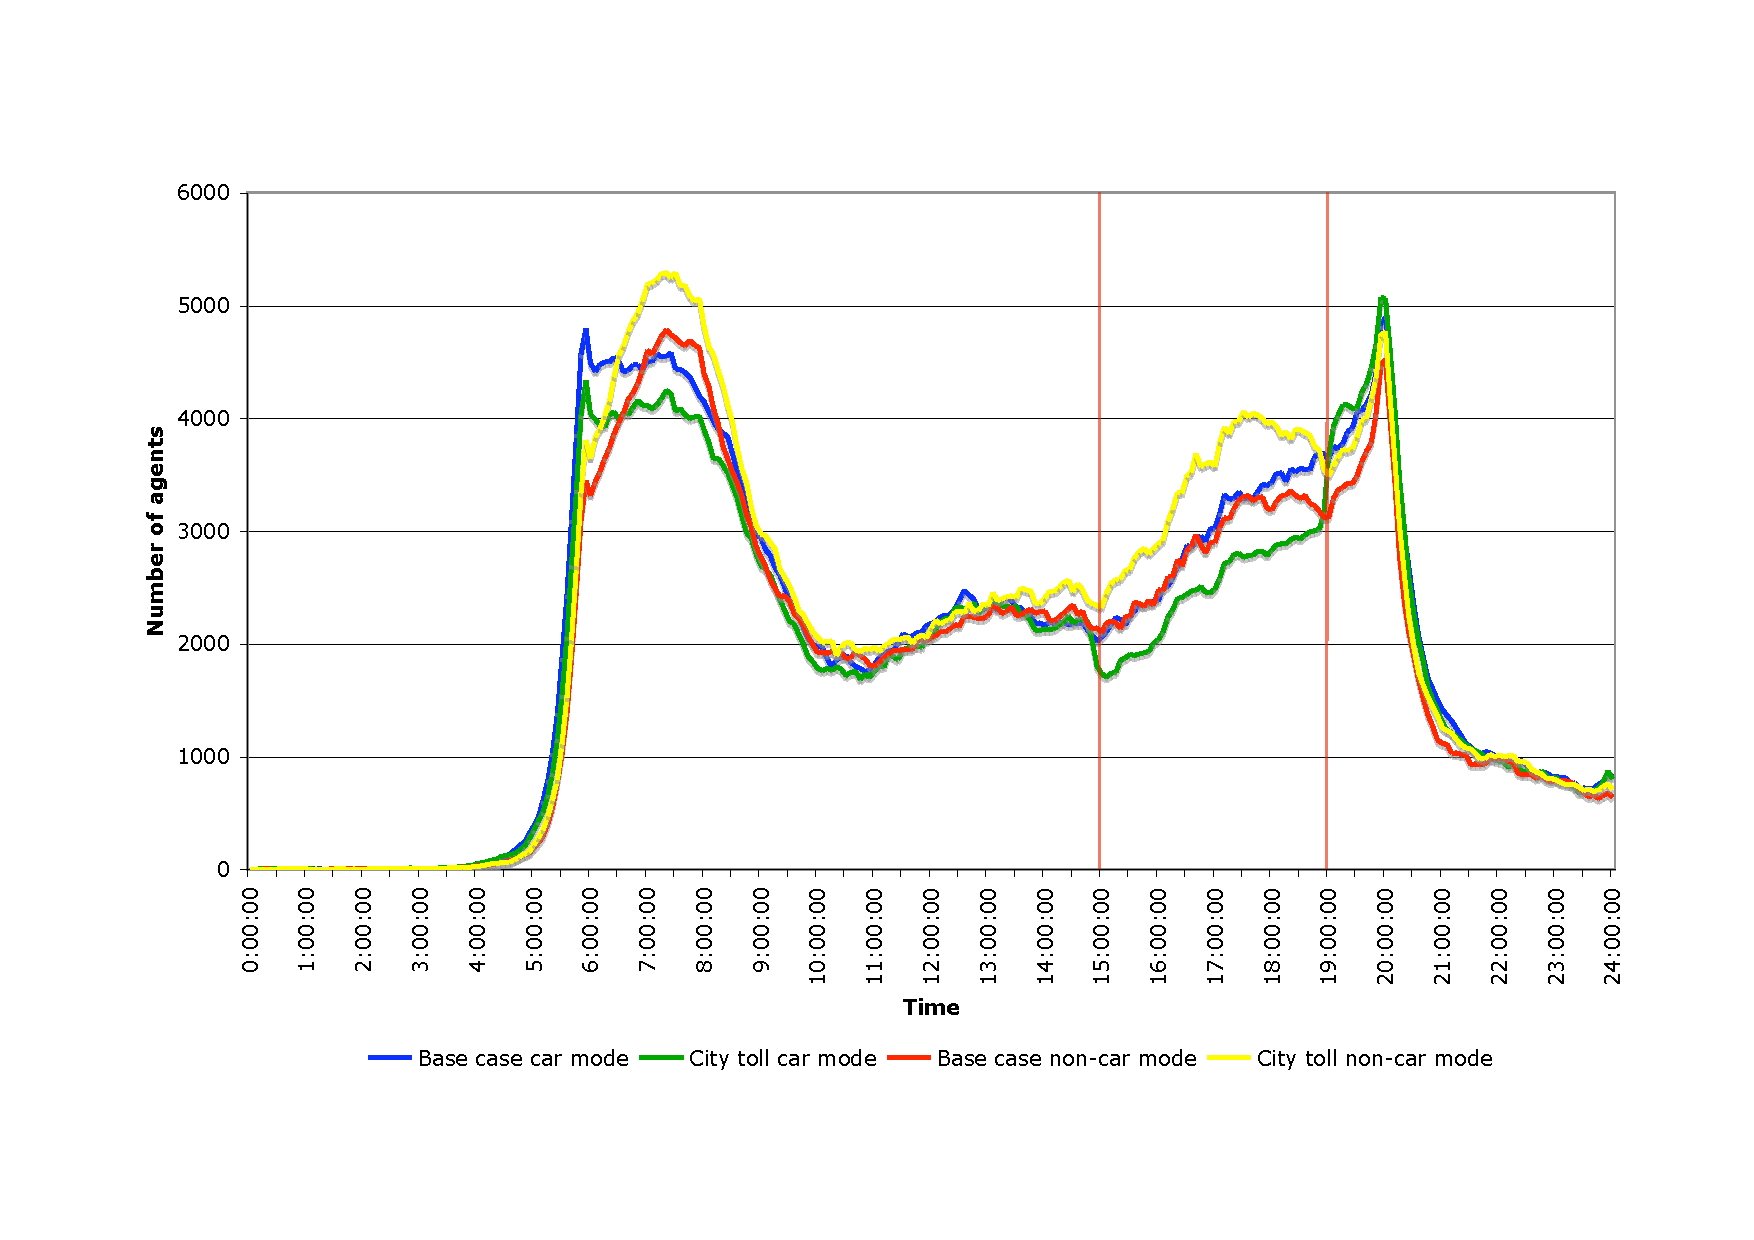
\includegraphics[width=0.99\hsize,trim=2cm 2.5cm 2cm 3cm,clip]{extending/figures/roadpricing/583vs585onRoute.pdf}}%
{}
% ------------
%% \benjamin{Es gibt ein ähnliches Bild auch in meiner Diss...Verweis siehe unten.}
%% \benjamin{One could also cite NagelGretherEtc2008ag-based-evaluation...}

% ============================================================================
\subsection{Income-Dependent Values of Time}
Similar to \citet{RieserEtAl_TRBTDF_2008}, \citet{KickhoeferEtAl2010EconomicEvaluationPublicAcceptanceRoadPricingKuhmo, Kickhoefer_PhDThesis_2014} introduced a distance-based morning peak toll on the same links between 6:30\,am and 9:00\,am. Toll levels were increased stepwise from 0.28\,$CHF/km$ up to an almost prohibitive price of 44.80\,$CHF/km$. The studies assume an income-dependent utility functions with a decreasing marginal utility of money. The goal was to (i) identify the welfare-maximizing toll level which potentially is dependent on the aggregation rule of user benefits (see Chapter~\ref{ch:economicEval}), and (ii) to investigate the distributional aspects of such pricing schemes.
%
The studies showed that changes in travel patterns resulting from the morning peak toll triggered though the whole day, affecting traffic patterns in the afternoon.
%
Furthermore, the study showed that such a parametric approach is capable to identify the welfare-maximizing toll level. However, it was found that the level of the overall welfare effect highly depends on the aggregation rule for user benefits, i.e.,\,if one first monetizes individual utilities and then adds up, or first adds up utilities and then monetizes. 
Even the sign of that effect might not be stable depending on that choice.
%
For more information, please refer to the two studies above.

%% \kai{todo}
%% \benjamin{done?}

% ============================================================================
\subsection{Integrated Passenger and Freight Toll Simulation for the Gauteng Province in South Africa}
A large scale application was undertaken for the Gauteng province in South Africa (cf.\ Section~\ref{sec:gauteng}). It is based on the so-called e-toll, which was switched on in December 2013. The e-toll plausibly charges different rates for different vehicle types, charging higher rates for heavy trucks. Again plausibly, this should go along with higher values of time of the driver-vehicle-units.  Somewhat surprisingly, this turned out to be difficult to do with the \gls{matsim} software structure that was there when the project was started in 2008. While it was easy to charge the higher toll to the freight vehicles, it was difficult to give different replanning methods and a different scoring function to the freight population, and it was essentially impossible to feed the router with the different values of time of the freight population. This was an important driver for much development in recent years, including making the scoring function better accessible (cf.\ Section~\ref{sec:scoring-extension-point}), allowing different replanning strategies for different sub-populations (Section~\ref{sec:strategymodules}), 
%\kai{erwähnen wir die sub-populations irgendwo?}
 and reducing the consistency requirements between the router, the vehicle-based toll and the driver-based scoring function \citep{NagelKickhoeferJoubert2014HeterogeneousVoTsPROCEDIA}.

The simulation, as expected, predicts reduced traffic volumes on the tolled roads, and increased volumes elsewhere (Figure \ref{fig:gauteng-toll-volumes}).

% ------------
\createfigure%
{\kai{Better figure: logo?} Predicted differences in link volumes after introduction of the toll (red: higher volumes, green: lower volumes)}%
{\kai{Better figure: logo?} Predicted differences in link volumes after introduction of the toll (red: higher volumes, green: lower volumes)}%
{\label{fig:gauteng-toll-volumes}}%
{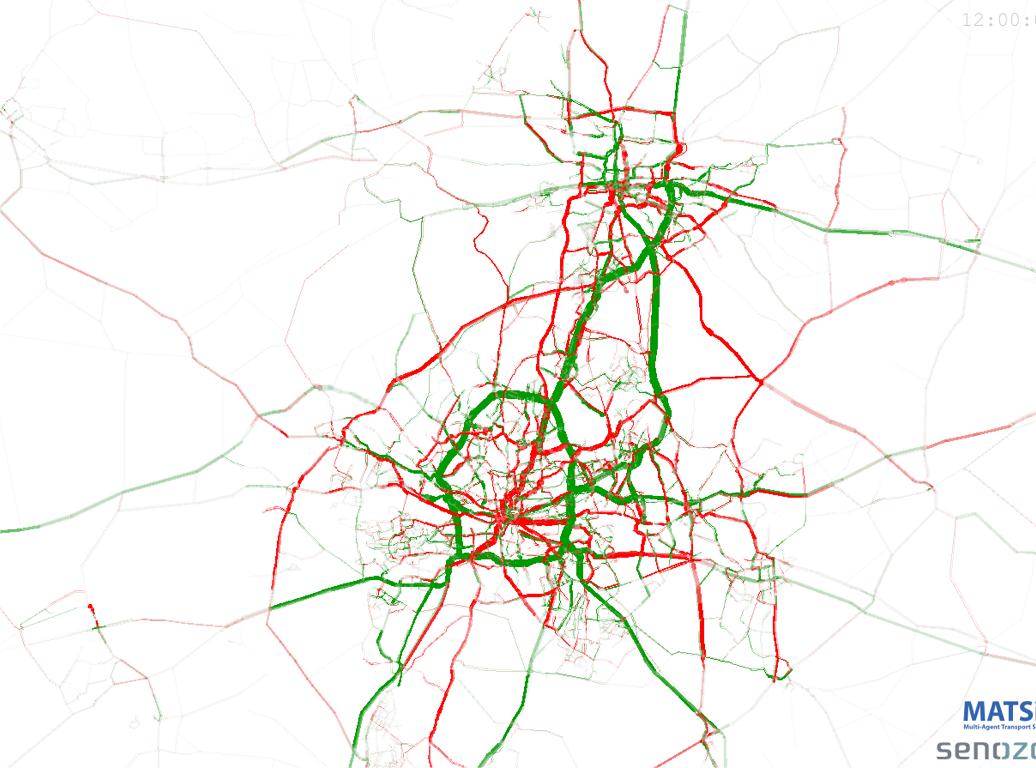
\includegraphics[width=0.8\hsize,trim=0 0 0 0,clip]{extending/figures/roadpricing/abs-diff-link-vol-vot55-24h.png}}%
{}
% ------------

% ##################################################################################################################
\section{Invocation}
\subsection{Minimal}
The least amount of infrastructure is necessary when running roadpricing from the command line. For this, the \gls{matsim} \gls{jar}, its libraries, \emph{and} the roadpricing \gls{jar} need to be downloaded either from a release or from the nightly builds (Section~\ref{sec:releases-builds}). After unzipping all zip files, the necessary command roughly is
\begin{lstlisting}
java -Xmx2000m -cp MATSim.jar:roadpricing-.../roadpricing-...jar org.matsim.roadpricing.run.RunRoadPricingExample config.xml  
\end{lstlisting}
where \lstinline$config.xml$ needs to contain a section
\begin{xml}
	<module name="roadpricing" >
		<param name="tollLinksFile" value="<path>/<tollfilename>" />
	</module>
\end{xml}
The toll file looks like this:
%
\begin{xml}
<roadpricing type="link" name="abc">
   <links>
      <link id="11">
         <cost start_time="05:00" end_time="10:00" amount="1." />
         <cost start_time="17:00" end_time="20:00" amount="1." />
      </link>             
      <link id="12" />
   </links>

   <!--this is for all links with no cost entry above:-->
   <cost start_time="05:00" end_time="10:00" amount="2.00"/>

</roadpricing>
\end{xml}
%
As one can see, there is a section where each link can be entered separately. There can also be a separate cost structure for each link. All links that are listed, but without a cost structure, fall back on the general cost structure listed at the end. Links which are not listed are without toll.

% ============================================================================
\subsection{Toll Schemes}
\paragraph{Link toll} The example refers to the "link" toll scheme, indicated by \lstinline$type="link"$.  It charges the amount that is specified on the link.

\paragraph{Distance toll} Another useful scheme is "distance", indicated by \lstinline$type="distance"$.  Here, the \lstinline$amount$ is interpreted as amount per length unit (cf.\ Section~\ref{sec:unitsconventions}). This is most useful with only a list of tolled links, and a uniform distance cost for all these links noted at the end of the file.

\paragraph{Area toll} The simulation of an \emph{area toll}---i.e.,\,a toll where one has to pay a flat fee for a given time period, often a day, once one drives anywhere inside the area---suffers from a combinatorial challenge: Driving through the tolled area early in the day may only pay off if one can re-use the permit later in the day. The code in principle addresses that by routing the agent twice: once under the assumption of a zero toll and once under the assumption of a very large toll. Afterward, the toll is added to the generalized cost of the first option, and then both options are compared.  
%
In the end, the approach suffered from the same consistency burden as the general approach (see end of Section~\ref{sec:roadpricing-intro}): The router made the decision about which variant was better rather than leaving the decision to the agent. It should be re-implemented using the same principles as used by \citet{NagelKickhoeferJoubert2014HeterogeneousVoTsPROCEDIA}.

\paragraph{Cordon toll} The cordon toll scheme was derived from the area scheme, in the sense that one could use the same file that listed all links in the area also for the cordon toll. The code made sure that toll was only charged when a vehicle moved from an untolled link to a tolled link---thereby effectively crossing the cordon. A challenge with this approach is that it is confusing if there is not a connected area and instead several links in sequence are tolled.  Then, if these links are connected, the toll is only charged on the first of them; if there is a small section missing, maybe because it was overlooked, then the toll is charged again. 

% ============================================================================
%\subsection{Invocation as "Script in Java"}

%See Sec.~\ref{sec:roadpricing-stdInfo} under "Invoking the module".

%% The above \lstinline$org.matsim.roadpricing.run.Main$ class can also be used as a starting point for one's own ``script in Java'':
%% \begin{lstlisting}
%% public static void main(String[] args) {
%% 	// load the config, telling it to "materialize" the road pricing section:
%% 	Config config = ConfigUtils.loadConfig(args[0], new RoadPricingConfigGroup());
	
%% 	// load the scenario:
%% 	Scenario scenario = ScenarioUtils.loadScenario(config) ;

%% 	// instantiate the controler:
%% 	Controler controler = new Controler(scenario) ;

%% 	// instantiate road pricing and add it as controler listener:
%% 	RoadPricing roadPricing = new RoadPricing() ;
%% 	controler.addControlerListener( roadPricing ) ;

%% 	// run the controler:
%% 	controler.run() ;
%% }
%% \end{lstlisting}

% ##################################################################################################################
%\section{More information}

%See Sec.~\ref{sec:roadpricing-stdInfo}.

%% \url{http://ci.matsim.org:8080/job/MATSim_contrib_M2/org.matsim.contrib$roadpricing/javadoc/?}

% ##################################################################################################################
% Local Variables:
% mode: latex
% mode: reftex
% mode: visual-line
% TeX-master: "../../main"
% comment-padding: 1
% fill-column: 9999
% End: 
